\chapter{تشخیص و تصحیح خطا در پارامترهای مدل نورونی} \label{chap:errors}

در این فصل، ابتدا با استفاده از تقریب بته\LTRfootnote{Bethe approximation} و الگوریتم انتشار باور\LTRfootnote{Belief propagation}، آنتروپی را به عنوان سنجه‌ای برای تعداد جواب‌های دینامیکی یک سیستم نورونی دارای خطا محاسبه کرده و تعداد این جواب‌های دینامیکی را تعیین می‌کنیم.
سپس، با بهره‌گیری از روش مونته‌کارلو\LTRfootnote{Monte Carlo method}، به تصحیح خطاهای موجود در پارامترهای مدل نورونی نگاشت چیالوو که در فصل قبل معرفی شد، می‌پردازیم.
در نهایت، نتایج به دست آمده را مورد بررسی قرار می‌دهیم.

\section{تعداد جواب‌های دینامیکی}
فرض کنید
\( \mathbf{r}^{*} \)،
یک دنباله مشاهده شده از دینامیک یک نورون سالم و بدون خطا با طول
\( \mathcal{T} \)
باشد:
\begin{equation}
    \mathbf{r}^{*} = \left\{ r^{*}_{t} \right\}_{t=1}^{\mathcal{T}} = \left\{ \left( x_{1}^{*}, y_{1}^{*} \right) , \left( x_{2}^{*}, y_{2}^{*} \right), \ldots, \left( x_{\mathcal{T}}^{*}, y_{\mathcal{T}}^{*} \right) \right\}
\end{equation}
حال اگر نورون دچار خطا و بیماری شود، دنباله
\( \mathbf{r} \)
مشاهده خواهد شد:
\begin{equation}
    \mathbf{r} = \left\{ r_{t} \right\}_{t=1}^{\mathcal{T}} = \left\{ \left( x_{1}, y_{1} \right) , \left( x_{2}, y_{2} \right), \ldots, \left( x_{\mathcal{T}}, y_{\mathcal{T}} \right) \right\}
\end{equation}
برای تشخیص و ارزیابی خطای وارد شده به نورون، می‌توان خطای میانگین توان دوم \LTRfootnote{Mean squared error} را به عنوان معیاری برای اندازه‌گیری فاصله‌ی بین دنباله‌های مشاهده شده و دنباله مرجع استفاده کرد.
این فاصله را می‌توان به صورت زیر تعریف کرد:
\begin{equation} \label{eq:mse}
    \text{MSE}(\mathbf{r}) = \frac{1}{\mathcal{T}} \sum_{t=1}^{\mathcal{T}} |r_{t} - r^{*}_{t}|^{2} = \frac{1}{\mathcal{T}} \sum_{t=1}^{\mathcal{T}} \left[ (x_{t} - x^{*}_{t})^{2} + (y_{t} - y^{*}_{t})^{2} \right]
\end{equation}
در اینجا،
\( r_{t} = (x_{t}, y_{t}) \) و \( r^{*}_{t} = (x^{*}_{t}, y^{*}_{t}) \)
به ترتیب نشان دهنده‌ی مقدار مشاهده شده‌ی دنباله‌ی
\( \mathbf{r} \)
و مقدار دنباله‌ی مرجع در زمان
\( t \)
است.

مسئله‌ی اساسی این است که در صورت وقوع خطا در نورون و مشاهده دینامیکی متفاوت که فاصله‌ی مشخصی از دینامیک نورون سالم دارد، چه تعداد دینامیک متفاوت دیگر ممکن است وجود داشته باشد که همان فاصله را از دینامیک نورون سالم دارند؟
به عبارت دیگر، در صورتی که نورون دچار خطا شود و دنباله‌هایی تولید کند که فاصله‌ای مشخص از دنباله‌ی مرجع دارند، تعداد جواب دینامیکی ممکن با همین فاصله چقدر است؟

برای پاسخ به این پرسش و تعیین تعداد حالت‌ها و جواب‌های دینامیکی ممکن برای دنباله‌ی مشاهده شده
\( \mathbf{r} \)
از یک نورون بیمار، می‌توان از ابزارهایی که فیزیک آماری در اختیار ما قرار داده است، بهره برد.
فیزیک آماری با معرفی چارچوب‌هایی برای محاسبه انرژی و آنتروپی یک سیستم با استفاده از تابع پارش، به ما امکان می‌دهد تا اطلاعاتی درباره تعداد حالت‌های ممکن در دسترس سیستم به دست بیاوریم.
یکی از این چارچوب‌های احتمالاتی، آنسامبل کانونی است که بر روی فضای همه حالت‌های ممکن سیستم تعریف می‌شود و از توزیع بولتزمن-گیبز پیروی می‌کند.

برای محاسبه‌ی تابع پارش سیستم در آنسامبل کانونی، لازم است احتمال رخداد هر دنباله را بدانیم.
بنابراین، احتمال رخداد دنباله
\( \mathbf{r} \)
را به شکل زیر تعریف می‌کنیم:
\begin{equation} \label{eq:probability}
    P(\mathbf{r}) = \frac{1}{Z_{\mathcal{T}}(\beta)} e^{-\beta E(\mathbf{r})} \prod_{t=2}^{\mathcal{T}} \delta(f(r_{t}), r_{t+1})
\end{equation}
در این معادله
\( Z_{\mathcal{T}}(\beta) \)
یک ثابت بهنجارش است که با نام تابع پارش شناخته می‌شود و به شکل زیر تعریف می‌شود:
\begin{equation}
    Z_{\mathcal{T}}(\beta) = \sum_{\{ \mathbf{r} \}} e^{-\beta E(\mathbf{r})} \prod_{t=2}^{\mathcal{T}} \delta(f(r_{t}), r_{t+1})
\end{equation}
در اینجا،
\( E(\mathbf{r}) \)
تابع انرژی سیستم است که به فاصله‌ی بین دنباله‌های مشاهده شده
\( \mathbf{r} \) و \( \mathbf{r}^{*} \)
بستگی دارد و به شکل زیر تعریف می‌شود:
\begin{equation}
    E(\mathbf{r}) = \sum_{t=1}^{\mathcal{T}} |r_{t} - r^{*}_{t}|^{2}
\end{equation}
پارامتر
\( \beta \)
نیز پارامتری کنترلی است که فاصله‌ی بین دو دنباله‌ی مشاهده شده را تنظیم می‌کند و معادل با معکوس دما در سیستم‌های ترمودینامیکی است.
تابع
\( \delta(f(r_{t}), r_{t+1}) \)،
تابع دلتای دیراک است که برای اعمال قیدهای دینامیکی نورون در
\( P(\mathbf{r}) \)
وارد شده است.
همچنین، تابع
\( f(r_{t}) \)
با اعمال نگاشت چیالوو، مقدار
\( r_{t+1} \)
را بر اساس
\( r_{t} \)
محاسبه می‌کند.

در فیزیک آماری، برای هر سیستم می‌توان مفاهیم انرژی و آنتروپی را تعریف و محاسبه کرد.
اما انرژی و آنتروپی در سیستم موردنظر ما چه مفهومی دارند؟
در اینجا، انرژی سیستم برابر با میانگین فاصله‌ی بین دنباله‌ی مرجع و تمامی دنباله‌هایی است که سیستم، با در نظر گرفتن قید‌های دینامیکی، می‌تواند از خود نشان دهد.
به عبارت دیگر، این انرژی نشان دهنده‌ی میانگین فاصله‌ی دنباله‌های دینامیکی مشاهده شده از دنباله‌ی مرجع است.

همچنین، آنتروپی سیستم بیانگر تعداد حالت‌های ممکن برای سیستم است که در یک
\( \beta \)
با مقدار مشخص، فاصله‌ای معین از دنباله‌ی مرجع دارند.
به بیان ساده‌تر، آنتروپی در این سیستم معیاری برای شمارش تمامی دنباله‌هایی است که میانگین انرژی معینی دارند.

همان‌طور که از فیزیک آماری می‌دانیم، برای به دست آوردن انرژی و آنتروپی یک سیستم، لازم است انرژی آزاد یا آنتروپی آزاد آن سیستم را محاسبه کنیم.
با دانستن انرژی آزاد یا آنتروپی آزاد سیستم می‌توان به ویژگی‌های مهم ماکروسکوپی هر سیستم آماری دسترسی پیدا کرد.
چگالی آنتروپی آزاد برای یک سیستم به صورت زیر تعریف می‌شود:
\begin{equation}
    \Phi_{\mathcal{T}}(\beta) = -\beta F_{\mathcal{T}}(\beta) = \frac{1}{\mathcal{T}} \ln Z_{\mathcal{T}}(\beta)
\end{equation}
در اینجا،
\( F_{\mathcal{T}}(\beta) \)
چگالی انرژی آزاد و
\( Z_{\mathcal{T}}(\beta) \)
تابع پارش سیستم است.

دو کمیت مهم فیزیکی، چگالی انرژی و چگالی آنتروپی هستند که به صورت مشتق‌هایی از چگالی انرژی آزاد تعریف می‌شوند:
\begin{equation*}
    E_{\mathcal{T}}(\beta) = \frac{\partial}{\partial \beta} (\beta F_{\mathcal{T}}(\beta)), \qquad S_{\mathcal{T}}(\beta) = \beta^{2} \frac{\partial F_{\mathcal{T}}(\beta)}{\partial \beta}
\end{equation*}
همچنین، می‌توان نشان داد که این دو رابطه، در معادله‌های زیر نیز صدق می‌کنند
\cite{mezard2009}:
\begin{equation}
    F_{\mathcal{T}}(\beta) = E_{\mathcal{T}}(\beta) - \frac{1}{\beta} S_{\mathcal{T}}(\beta)
\end{equation}
\begin{equation}
    \Phi_{\mathcal{T}}(\beta) = S_{\mathcal{T}}(\beta) - \beta E_{\mathcal{T}}(\beta)
\end{equation}

در فیزیک آماری، روش‌های متعددی برای محاسبه آنتروپی آزاد و همچنین میانگین انرژی و آنتروپی سیستم وجود دارد.
یکی از ساده‌ترین این روش‌ها، تقریب میدان میانگین است.
در این تقریب، اجزای سیستم به صورت مستقل از هم در نظر گرفته می‌شوند و اثرات برهمکنش‌ها به صورت یک میدان مؤثر یا میانگین، اعمال می‌شود، به طوری که فرض می‌شود هیچ برهمکنش مستقیمی بین اجزای سیستم وجود ندارد.
همچنین، در این روش، از افت‌وخیزهای همسایه‌های هر جز صرف‌نظر می‌شود و اثر همسایه‌ها با یک میانگین آماری جایگزین می‌شود.
این تقریب، هنگامی که همبستگی‌های اجزای سیستم تنها در فاصله‌های بسیار کوتاه اهمیت داشته و در فاصله‌های بلند قابل چشم‌پوشی باشند، به خوبی عمل کرده و نتایجی قابل قبول ارائه می‌دهد.
با این حال، در نقطه‌های بحرانی، جایی که همبستگی‌ها بلندبرد نقشی اساسی در سیستم دارند، این روش به خوبی عمل نمی‌کند
\cite{weiss1907,chandler1987,kadanoff2009}.

روش دیگر برای محاسبه آنتروپی آزاد، استفاده از روش مونته‌کارلو است.
در این روش، سیستم به صورت عددی شبیه‌سازی می‌شود و با ایجاد تغییر‌های متعدد در حالت‌های سیستم، آن را به عبور از حالت‌های مختلف وادار می‌کنند.
به طوری که احتمال وقوع هر حالت با توزیع حالت‌های ممکن در سیستم واقعی مطابقت داشته باشد.
این روش با شبیه‌سازی بخش کوچکی از حالت‌های در دسترس سیستم می‌تواند با دقت خوبی کمیت‌های فیزیکی را محاسبه کند.
با این حال، یکی از مشکل‌های اساسی این روش آن است که ممکن است تمامی حالت‌های مرتبط با سیستم در فرآیند شبیه‌سازی در نظر گرفته نشود.
این کمبود می‌تواند منجر به ایجاد خطا در تخمین مقدار میانگین‌های محاسبه شده شود و دقت نتایج را تحت تأثیر قرار دهد.
به عبارت دیگر، در بسیاری از موارد برای دستیابی به دقت موردنظر به زمان اجرای بسیار زیادی برای به تعادل رساندن سیستم و نمونه‌گیری نیاز داریم.
بنابراین، این روش در برخی موارد بسیار پرهزینه خواهد بود.
در اینجا نیز به دلیل نیاز به محاسبه‌ی آنتروپی سیستم، این روش هزینه‌ی محاسباتی بالایی دارد
\cite{newman1999,landau2021}.

تقریب بته نیز یکی دیگر از روش‌های محاسبه ویژگی‌های تعادلی سیستم از جمله میانگین انرژی و آنتروپی است که برای مسئله‌هایی با شبکه‌ی برهمکنشی تنک به خوبی عمل می‌کند.
در این تقریب، تنها همبستگی‌ها با همسایه‌ی اول در نظر گرفته می‌شوند و از همبستگی‌های با فاصله‌ی دورتر صرف‌نظر می‌شود.
بنابراین، اگر شبکه‌ی برهمکنش سیستم ساختاری درختی داشته باشد، این تقریب جوابی دقیق خواهد داشت
\cite{mezard2009}.

این تقریب در برخی از مسئله‌ها از روش مونته‌کارلو کارآمدتر و کم‌هزینه‌تر است.
همان‌طور که در ادامه نشان خواهیم داد و در
\autoref{fig:factor_graph}
مشاهده می‌کنید، شبکه‌ی برهمکنش‌های سیستم موردنظر ما ساختار درختی دارد.
بنابراین، استفاده از تقریب بته در اینجا انتخاب مناسبی است.
در ادامه، با بهره‌گیری از این تقریب به محاسبه‌ی میانگین انرژی و آنتروپی
سیستم خواهیم پرداخت.

احتمال رخداد دنباله
\( \mathbf{r} \)
را که در
\autoref{eq:probability}
معرفی شده است،
در نظر بگیرید.
می‌توانیم این احتمال را به فرم زیر بازنویسی کنیم:
\begin{equation} \label{eq:probability_product}
    P(\mathbf{r}) = \frac{1}{Z_{\mathcal{T}}(\beta)} \prod_{t=1}^{\mathcal{T}} \psi_{t}(r_{t}) \prod_{t=1}^{\mathcal{T}-1} \mathbbm{1}(r_{t}, r_{t+1})
\end{equation}
در این معادله،
\( \psi_{t}(r_{t}) = \exp \left( {-\beta |r_{t} - r^{*}_{t}|^{2}} \right) \)
یک تابع نمایی از فاصله‌ی بین حالت مشاهده شده
\( r_{t} \)
و حالت مرجع
\( r^{*}_{t} \)
در زمان
\( t \)
است.
تابع
\( \mathbbm{1}(r_{t}, r_{t+1}) = \delta(f(r_{t}), r_{t+1}) \)
نیز، یک تابع دلتای دیراک است که برای اعمال قیدهای دینامیکی بین حالت‌های متوالی
\( r_{t} \) و \( r_{t+1} \)
وارد معادله شده است.

\begin{figure}
    \centering
    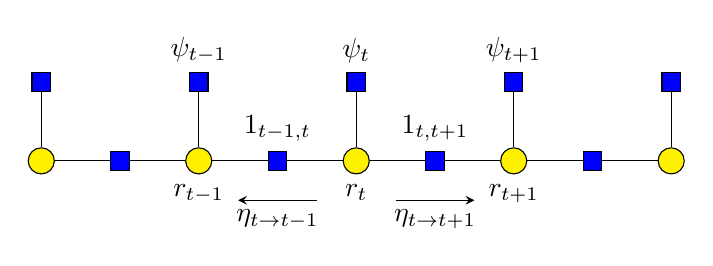
\begin{tikzpicture}[>=stealth]
        \node[circle, draw, fill=yellow] (A) at (0,0) {};
        \node[rectangle, draw, fill=blue] (B) at (1,0) {};
        \node[circle, draw, fill=yellow, label=below:\( r_{t-1} \)] (C) at (2,0) {};
        \node[rectangle, draw, fill=blue, label=above:\( \mathbbm{1}_{t-1, t} \)] (D) at (3,0) {};
        \node[circle, draw, fill=yellow, label=below:\( r_{t} \)] (E) at (4,0) {};
        \node[rectangle, draw, fill=blue, label=above:\( \mathbbm{1}_{t, t+1} \)] (F) at (5,0) {};
        \node[circle, draw, fill=yellow, label=below:\( r_{t+1} \)] (G) at (6,0) {};
        \node[rectangle, draw, fill=blue] (H) at (7,0) {};
        \node[circle, draw, fill=yellow] (I) at (8,0) {};
        \node[rectangle, draw, fill=blue] (J) at (0,1) {};
        \node[rectangle, draw, fill=blue, label=above:\( \psi_{t-1} \)] (K) at (2,1) {};
        \node[rectangle, draw, fill=blue, label=above:\( \psi_{t} \)] (L) at (4,1) {};
        \node[rectangle, draw, fill=blue, label=above:\( \psi_{t+1} \)] (M) at (6,1) {};
        \node[rectangle, draw, fill=blue] (N) at (8,1) {};

        \draw[-] (A) -- (B);
        \draw[-] (B) -- (C);
        \draw[-] (C) -- (D);
        \draw[-] (D) -- (E);
        \draw[-] (E) -- (F);
        \draw[-] (F) -- (G);
        \draw[-] (G) -- (H);
        \draw[-] (H) -- (I);
        \draw[-] (A) -- (J);
        \draw[-] (C) -- (K);
        \draw[-] (E) -- (L);
        \draw[-] (G) -- (M);
        \draw[-] (I) -- (N);

        \draw[->] (4.5,-0.5) -- (5.5,-0.5) node[midway, below] {\( \eta_{t \to t+1} \)};
        \draw[<-] (2.5,-0.5) -- (3.5,-0.5) node[midway, below] {\( \eta_{t \to t-1} \)};
    \end{tikzpicture}
    \caption[
        شبکه برهمکنش متغیرهای
        \( r_{t} \)
        و قیدهای حاکم بر این متغیر‌ها
    ]
    {
        شبکه برهمکنش متغیرهای
        \( r_{t} \)
        و قیدهای حاکم بر این متغیر‌ها. گره‌های دایره‌ای زرد نشان‌دهنده گره‌های متغیر و گره‌های مربعی آبی نشان‌دهنده گره‌های قیدی حاکم بر متغیرهای
        \( r_{t} \)
        است.
    }
    \label{fig:factor_graph}
\end{figure}

همان‌طور که در
\autoref{fig:factor_graph}
مشاهده می‌کنید، می‌توان
\autoref{eq:probability_product}
را به شکل شبکه‌ای از برهمکنش‌های بین اجزای سیستم نمایش داد.
این شبکه شامل گره‌های متغیر
\( r_{t} \)
است که با دایره‌های زرد مشخص شده‌اند
و گره‌های قیدی
\( \psi_{t}(r_{t}) \) و \( \mathbbm{1}(r_{t}, r_{t+1}) \)
مربع‌های آبی هستند که محدودیت‌های دینامیکی و احتمالاتی را بر روی گره‌های متغیر اعمال می‌کنند.

نمایش تابع احتمال
\( P(\mathbf{r}) \)
به شکل بالا، نشان‌دهنده‌ی کارکرد مناسب تقریب بته در تحلیل و بررسی تعداد جواب‌های دینامیکی این سیستم است.
با استفاده از این تقریب، می‌توان احتمال رخداد حالت
\( r_{t} \)
در هر گره را به صورت ضرب احتمال حالت‌های همسایه‌های آن گره بیان کرد.
در نتیجه، می‌توان معادله‌های زیر را برای تابع توزیع احتمال حاشیه‌ای هر متغیر نوشت.

تابع توزیع احتمال حاشیه‌ای برای متغیر
\( r_{t} \)
در غیاب برهمکنش بین گره‌های
\( r_{t} \) و \( r_{t+1} \)
به شکل زیر بیان می‌شود:
\begin{equation} \label{eq:bp_constraint}
    \eta_{t \to t+1}(r_{t}) = \frac{\psi_{t}(r_{t})}{z_{t \to t+1}} \sum_{r_{t-1}} \eta_{t-1 \to t}(r_{t-1}) \mathbbm{1}(r_{t-1},r_{t})
\end{equation}
این معادله نشان می‌دهد که توزیع احتمال حاشیه‌ای برای متغیر
\( r_{t} \)
هنگامی که متغیر
\( r_{t+1} \)
و تمام همسایه‌های آن به جز متغیر
\( r_{t} \)
از شبکه‌ی برهمکنش‌ها حذف شده باشند را
می‌توان به صورت ضرب احتمال رخداد حالت
\( r_{t} \)،
یعنی
\( \psi(r_{t}) \)
که از تابع توزیع بولتزمن پیروی می‌کند و
احتمال‌های حاشیه‌ای مربوط به همسایه‌های
\( r_{t} \)، یعنی
\( \eta_{t-1 \to t}(r_{t-1}) \)
و قید‌های دینامیکی مدل دینامیکی، یعنی
\( \mathbbm{1}(r_{t-1},r_{t}) \)،
بیان کرد.

با توجه به رابطه بالا، می‌توان
توزیع احتمال حاشیه‌ای برای متغیر
\( r_{t} \)
با در نظر گرفتن همه‌ی همسایه‌ها
به شکل زیر بیان کرد:
\begin{equation} \label{eq:bp_variable}
    \eta_{t}(r_{t}) = \frac{\psi_{t}(r_{t})}{z_{t}} \left( \sum_{r_{t-1}} \eta_{t-1 \to t}(r_{t-1}) \mathbbm{1}(r_{t-1},r_{t}) \right) \left( \sum_{r_{t+1}} \eta_{t+1 \to t}(r_{t+1}) \mathbbm{1}(r_{t},r_{t+1}) \right)
\end{equation}

همچنین، ثابت‌های بهنجارش
\( z_{t \to t+1} \) و \( z_{t} \)
که در معادله‌های
\ref{eq:bp_constraint} و \ref{eq:bp_variable}
آمده‌اند، به صورت زیر تعریف می‌شوند:
\begin{equation} \label{eq:bp_normalization_constraint}
    z_{t \to t+1} = \sum_{r_{t}} \psi_{t}(r_{t}) \sum_{r_{t-1}} \eta_{t-1 \to t} \mathbbm{1}(r_{t-1},r_{t})
\end{equation}
\begin{equation} \label{eq:bp_normalization_variable}
    z_{t} = \sum_{r_{t}} \psi_{t}(r_{t}) \left( \sum_{r_{t-1}} \eta_{t-1 \to t}(r_{t-1}) \mathbbm{1}(r_{t-1},r_{t}) \right) \left( \sum_{r_{t+1}} \eta_{t+1 \to t}(r_{t+1}) \mathbbm{1}(r_{t},r_{t+1}) \right)
\end{equation}

تابع توزیع‌های احتمال حاشیه‌ای که توسط معادله‌های
\ref{eq:bp_constraint} و \ref{eq:bp_variable}
توصیف می‌شوند را می‌توان به شکل پیام‌هایی تعبیر کرد که بین متغیرها رد و بدل می‌شوند.
به همین دلیل، این معادله‌ها به نام معادله‌های انتشار باور نیز شناخته می‌شوند.
حالت کلی این معادله‌ها و روش به دست آوردن آن‌ها در
\ref{app:belief_propagation}
آمده است.
\cite{yedidia2005,mezard2009,zdeborova2016}.

با دانستن توزیع‌های احتمال حاشیه‌ای می‌توان چگالی آنتروپی آزاد و در نتیجه میانگین انرژی و آنتروپی سیستم را محاسبه کرد.
برای این منظور، یعنی یافتن جواب‌های تابع توزیع‌های احتمال حاشیه‌ای، می‌توان از الگوریتم انتشار باور استفاده کرد.
در زیر شبه کد این الگوریتم آورده شده است
\cite{zdeborova2016}.
\begin{algorithm}[H]
    \caption{الگوریتم انتشار باور}
    \begin{algorithmic}[1]
        \STATE \( \eta_{t \to t+1}(r_{t}) \)
        را با مقدار‌هایی تصادفی مقداردهی کنید.
        \STATE \( \eta_{t \to t+1}(r_{t}) \)
        را با استفاده از
        \autoref{eq:bp_constraint}
        به‌روزرسانی کنید.
        \STATE گام ۲ را تا همگرا شدن
        \( \eta_{t \to t+1}(r_{t}) \)
        به یک مقدار ثابت تکرار کنید.
        \STATE \( \eta_{t}(r_{t}) \)
        را محاسبه کنید.
    \end{algorithmic}
\end{algorithm}

پس از به دست آوردن احتمال‌های حاشیه‌ای، می‌توان از آن‌ها برای محاسبه‌ی چگالی آنتروپی آزاد استفاده کرد.
چگالی آنتروپی آزاد محاسبه شده از احتمال‌های حاشیه‌ای، به عنوان آنتروپی آزاد بته شناخته می‌شود و به صورت زیر محاسبه می‌شود:
\begin{equation} \label{eq:bethe_free_energy}
    \Phi = \frac{1}{\mathcal{\mathcal{T}}} \ln Z = \frac{1}{\mathcal{\mathcal{T}}} \left( \sum_{t=1}^{\mathcal{\mathcal{T}}} \ln z_{t} - \sum_{t=1}^{\mathcal{\mathcal{T}}-1} \ln z_{t,t+1} \right)
\end{equation}
در اینجا،
\( z_{t} \)
سهم متغیر
\( r_{t} \)
در تابع پارش است که تغییر در تابع پارش را هنگام اضافه شدن متغیر
\( r_{t} \)
و برهمکنش‌های مرتبط با آن به سیستم توصیف می‌کند و توسط
\autoref{eq:bp_normalization_variable}
داده می‌شود.
همچنین،
\( z_{t,t+1} \)
سهم برهمکنش‌های بین متغیرهای
\( r_{t} \) و \( r_{t+1} \)
است و تغییر در تابع پارش را هنگام اضافه شدن این برهمکنش‌ها به سیستم توصیف می‌کند.
این مقدار به صورت زیر به دست می‌آید:
\begin{equation} \label{eq:partial_partition_function}
    z_{t,t+1} = \sum_{r_{t}} \sum_{r_{t+1}} \eta_{t \to t+1}(r_{t}) \eta_{t+1 \to t}(r_{t+1}) \mathbbm{1}(r_{t},r_{t+1})
\end{equation}
در این معادله
\( \eta_{t \to t+1}(r_{t}) \) و \( \eta_{t+1 \to t}(r_{t+1}) \)
جواب‌های
\autoref{eq:bp_constraint}
هستند.

\autoref{eq:bethe_free_energy}
در واقع مجموع آنتروپی آزاد همه‌ی متغیرها را توصیف می‌کند.
اما از آنجا که در این مجموع هر برهمکنش دو بار شمارش می‌شود، برای تصحیح این شمارش اضافی، آنتروپی آزاد مربوط به برهمکنش‌ها از مجموع کسر می‌شود.
\cite{mezard2003}.

با این حال، حل معادله‌های انتشار باور و یافتن جواب‌های این معادله‌ها در اینجا به صورت تحلیلی ممکن نیست.
علاوه بر این، محاسبه‌ی عددی جواب‌های معادله‌های انتشار باور به دلیل پیوسته بودن فضای
\( r \)
دشوار است و نیاز به گسسته‌سازی فضای
\( r \)
دارد که این باعث افزایش حجم محاسبات می‌شود.
در نتیجه، استفاده از روش های عددی دیگر، نظیر روش دینامیک جمعیت\LTRfootnote{Population dynamics} به عنوان روشی مناسب برای حل این مسئله و یافتن جواب‌های معادله‌های انتشار باور به صورت تقریبی پیشنهاد می‌شود
\cite{mezard2001}.

روش دینامیک جمعیت به این صورت عمل می‌کند که توزیع‌های احتمال حاشیه‌ای را به شکل جمعیتی از مقدار‌های
\( r_{i} \)
در نظر می‌گیرد.
این جمعیت‌ها از طریق به‌روزرسانی بر اساس دینامیک سیستم موردنظر ما، یعنی نگاشت چیالوو و مقایسه انرژی آن‌ها، به سمت جواب‌های پایای توزیع‌های احتمال حاشیه‌ای هدایت می‌شوند.
در نهایت، با استفاده از این جمعیت‌ها، آنتروپی آزاد و آنتروپی سیستم محاسبه می‌شود.
شبه کد الگوریتم دینامیک جمعیت را به شکل زیر آورده شده است:
\begin{algorithm}[H]
    \caption{الگوریتم دینامیک جمعیت}
    \begin{algorithmic}[1]
        \STATE \( \eta_{t \to t+1} \)
        را با مقدار‌هایی تصادفی مقداردهی کنید.
        \STATE به صورت تصادفی
        \( r_{i} \)
        را از جمعیت
        \( \eta_{t-1 \to t} \) و \( r_{j} \)
        را از جمعیت
        \( \eta_{t \to t+1} \)
        انتخاب کنید.
        \STATE مقدار
        \( r_{\text{new}} = f(r_{i}) \)
        را محاسبه کرده و انرژی آن،
        \( E(r_{\text{new}}) \)،
        را تعیین کنید.
        \STATE اگر
        \( E(r_{\text{new}}) < E(r_{j}) \)
        شد،
        \( r_{\text{new}} \)
        را جایگزین
        \( r_{j} \)
        در جمعیت
        \( \eta_{t \to t+1} \)
        کنید.
        \STATE اگر
        \( E(r_{\text{new}}) > E(r_{j}) \)
        شد، با احتمال
        \( e^{-\beta \Delta E} \)، \( r_{\text{new}} \)
        را جایگزین
        \( r_{j} \)
        در جمعیت
        \( \eta_{t \to t+1} \)
        کنید.
        \STATE گام‌های ۲ تا ۵ را تا همگرا شدن جمعیت‌
        \( \eta_{t \to t+1} \)
        به یک مقدار ثابت تکرار کنید.
        \STATE گام‌های ۱ تا ۶ را برای
        \( \eta_{t \to t-1} \)
        نیز تکرار کنید.
    \end{algorithmic}
\end{algorithm}

برای یافتن تعداد جواب‌های دینامیکی مسئله و همچنین برای محاسبه‌ی میانگین فاصله‌ها از دنباله مرجع، از الگوریتم انتشار باور و روش دینامیک جمعیت استفاده کردیم.
این شبیه‌سازی‌ها را برای محاسبه‌ی انرژی و آنتروپی دنباله‌های مشاهده شده از نگاشت چیالوو بر اساس دنباله مرجع مشخصی انجام دادیم.
در این شبیه‌سازی‌ها، تنها تفاوت در شرایط اولیه‌ی دنباله‌های مشاهده شده، یعنی
\( r_{0} = (x_{0}, y_{0}) \)
بوده است، در حالی که پارامترهای نگاشت چیالوو برای دو ناحیه زیر ثابت نگه داشته شده‌اند:
\begin{itemize}[label=-]
    \item مرز بین ناحیه غیربرانگیخته و برانگیخته با پارامتر‌های
          \( a = 0.89 \)، \( b = 0.60 \)، \( c = 0.28 \) و \( k = 0.030 \)
    \item مرز بین ناحیه غیربرانگیخته و آشوبناک با پارامترهای
          \( a = 0.89 \)، \( b = 0.18 \)، \( c = 0.28 \) و \( k = 0.023 \)
\end{itemize}
در این شبیه‌سازی‌ها، پارامتر
\( \beta \)
در بازه‌ای مشخص تغییر دادیم تا میانگین انرژی و آنتروپی سیستم برای دنباله‌هایی با طول‌های ۳ و ۶ محاسبه کنیم.
نتایج به دست آمده برای میانگین انرژی و آنتروپی این سیستم به شرح زیر نمایش داده شده‌اند:
\begin{itemize}[label=-]
    \item برای دنباله‌های با طول ۳، نتایج در
          \autoref{fig:bp_3}
          نمایش داده شده‌اند.
    \item برای دنباله‌های با طول ۶، نتایج در
          \autoref{fig:bp_6}
          نمایش داده شده‌اند.
\end{itemize}

\begin{figure}
    \centering
    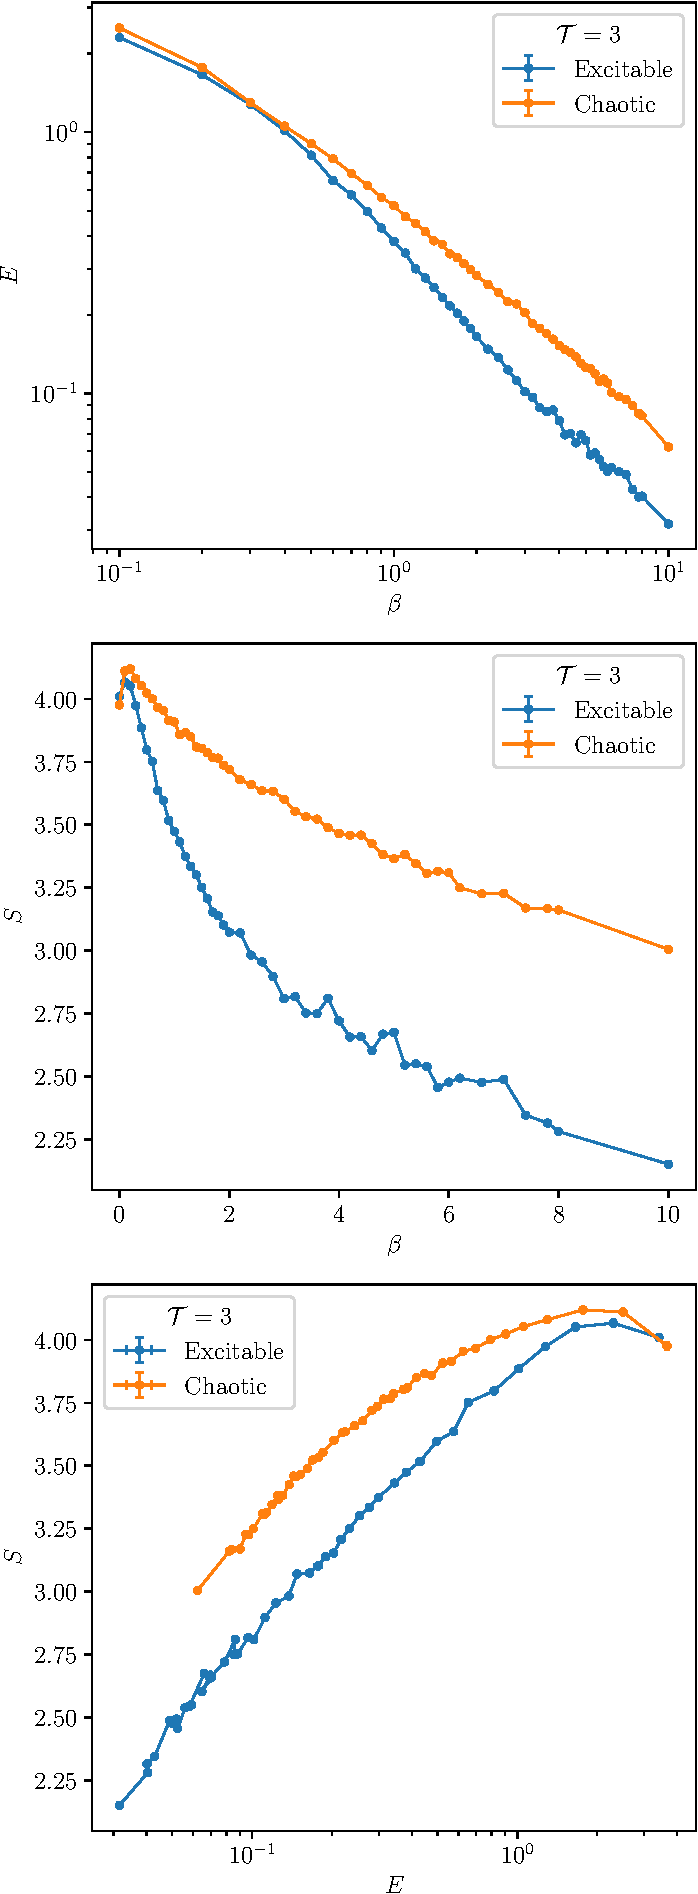
\includegraphics[height=0.9\textheight]{figures/bp_3}
    \caption{
        رفتار میانگین انرژی و آنتروپی نسبت به تغییر پارامتر
        \( \beta \)
        برای دنباله‌هایی با طول ۳
    }
    \label{fig:bp_3}
\end{figure}

همان‌طور که در
\autoref{fig:bp_3}
مشاهده می‌کنید، رفتار آنتروپی برای دنباله‌های با طول ۳ به گونه‌ای است که مقدار آنتروپی و تعداد جواب‌های دینامیکی در هر دو ناحیه‌ی مرز ناحیه برانگیخته و مرز ناحیه آشوبناک به خوبی از هم متمایز شده‌اند.
در این شکل می‌بینیم که تعداد جواب‌های دینامیکی در مرز ناحیه برانگیخته کمتر از مرز ناحیه آشوبناک است.
همچنین، با افزایش پارامتر
\( \beta \)،
تعداد جواب‌های دینامیکی در مرز ناحیه برانگیخته با شیب بیشتری نسبت به مرز ناحیه آشوبناک کاهش می‌یابند.
علاوه بر این، یک رفتار غیرمتعارف در آنتروپی نسبت به افزایش مقدار
\( \beta \)
و کاهش انرژی مشاهده می‌شود که در ادامه به تحلیل دقیق‌تر آن خواهیم پرداخت.

\begin{figure}
    \centering
    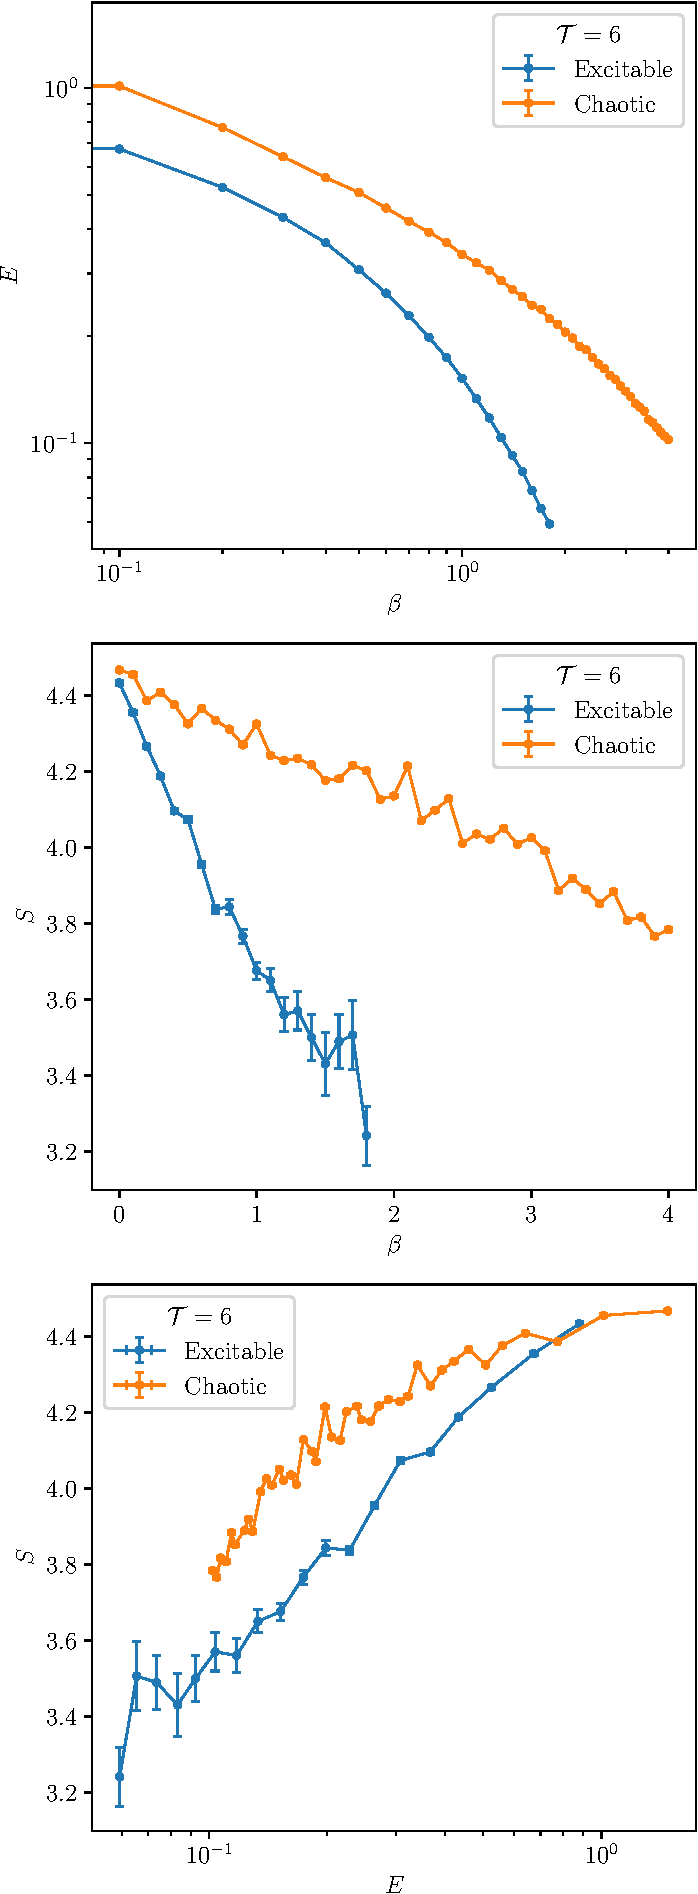
\includegraphics[height=0.9\textheight]{figures/bp_6}
    \caption{
        رفتار میانگین انرژی و آنتروپی نسبت به تغییر پارامتر
        \( \beta \)
        برای دنباله‌هایی با طول ۶
    }
    \label{fig:bp_6}
\end{figure}

در
\autoref{fig:bp_6}
رفتار میانگین انرژی و آنتروپی را برای دنباله‌هایی با طول ۶ مشاهده می‌کنید.
رفتار میانگین انرژی و آنتروپی در این طول نیز مشابه رفتار آن‌ها در طول ۳ است.
با این حال، با افزایش طول دنباله‌ی مشاهده شده، تعداد جواب‌های دینامیکی یا همان آنتروپی برای تمام مقدارهای
\( \beta \)
افزایش یافته است.
همچنین، رفتار غیرمتعارفی که در طول ۳ مشاهده می‌شد، در اینجا مشاهده نمی‌شود.

همان‌طور که گفته شد، در رفتار آنتروپی برای دنباله‌های با طول ۳،
\autoref{fig:bp_3}،
یک روند غیرمتعارف نسبت به پارامتر
\( \beta \)
و میانگین انرژی مشاهده می‌شود.
به این صورت که با افزایش
\( \beta \)
و کاهش انرژی، آنتروپی ابتدا افزایش یافته و سپس کاهش می‌یابد.
در حالی که انتظار می‌رود با کاهش انرژی، آنتروپی به طور یکنواخت کاهش یابد اما این رفتار در نتایج مشاهده نمی‌شود.

این رفتار غیرمتعارف ناشی از نحوه‌ی گسسته‌سازی پارامتر‌ها برای انجام شبیه‌سازی‌های عددی است.
می‌توان این رفتار را این گونه توضیح داد که در جایی که فاصله‌ی دنباله‌های مشاهده شده از دنباله مرجع زیاد است، با کاهش فاصله‌ی دنباله‌ها و میانگین انرژی، تعداد حالت‌هایی که قیدهای موجود در محاسبات عددی را برآورده می‌کنند، افزایش می‌یابند.
این افزایش در تعداد حالت‌های پذیرفته شده باعث افزایش آنتروپی و تعداد جواب‌های دینامیکی می‌شود.
با ادامه‌ی کاهش فاصله و میانگین انرژی، تعداد این حالت‌ها که تنها به دلیل قید‌های محاسبات عددی در سیستم وارد شده‌اند کاهش می‌یابند و رفتار آنتروپی به حالت مورد انتظار باز می‌گردد و کاهش می‌یابد.

\begin{figure}[!ht]
    \centering
    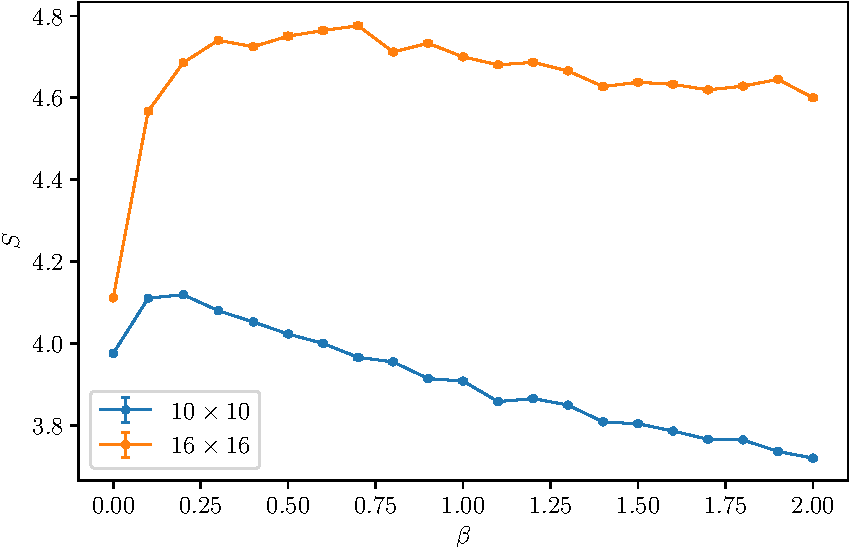
\includegraphics[width=0.8\textwidth]{figures/artifact}
    \caption{مقایسه رفتار غیرمتعارف آنتروپی برای دو نحوه‌ی متفاوت در گسسته‌سازی پارامترها}
    \label{fig:artifact}
\end{figure}

در
\autoref{fig:artifact}
این رفتار غیرمتعارف برای دو شبیه‌سازی با گسسته‌سازی‌های مختلف نشان داده شده است.
همان‌طور که مشاهده می‌کنید، با تغییر در نحوه‌ی گسسته‌سازی در محاسبه‌های عددی، این رفتار غیرمتعارف در آنتروپی بیشتر نمایان می‌شود.
به طوری که با افزایش تعداد نقاط گسسته‌سازی، مقدار آنتروپی در بازه‌ی بزرگ‌تری افزایش یافته است.
بنابراین، در شبیه‌سازی‌های بعدی باید این نکته را در نظر گرفت و پارامتر‌ها را به طور مناسب گسسته کرد.

\section{تصحیح خطا با روش مونته‌کارلو}
فرض کنید دنباله مرجع
\( \mathbf{r}^{*} \)
از یک نورون سالم مشاهده شده است.
نورون‌هایی بیمار وجود دارند که به دلیل خطا در پارامترهای خود، دنباله
\( \mathbf{r} \)
را تولید می‌کنند.
هدف ما این است که با تنظیم مناسب پارامترها، فاصله بین دنباله‌ی مرجع و دنباله‌ی مشاهده شده از نورون بیمار را کمینه کنیم.
یکی از روش‌های مناسب برای تصحیح این خطا و کمینه کردن فاصله بین دنباله‌ها، استفاده از روش مونته‌کارلو است.

معرفی و استفاده از روش‌های مونته‌کارلو به مقاله‌ی معروف متروپلیس و همکاران
\cite{metropolis1953}
بازمی‌گردد.
الگوریتم متروپلیس-هستینگز
\cite{metropolis1953,hastings1970}
بر اساس مقایسه‌ی هزینه‌ی اختلاف انرژی بین یک حالت از سیستم و همان حالت پس از ایجاد یک تغییر کوچک در آن حالت است.
اگر این تغییر باعث کاهش هزینه شود، پذیرفته می‌شود اما اگر هزینه افزایش یابد، تغییر با احتمالی متناسب با اختلاف هزینه پذیرفته خواهد شد.
این فرآیند با ایجاد تغییرهای کوچک، به طور پیوسته ادامه می‌یابد تا انرژی سیستم به یک مقدار کمینه برسد
\cite{newman1999,landau2021}.

یکی از مزیت‌های مهم روش‌های مبتنی بر مونته‌کارلو این است که اگر برای مدت زمان کافی، تغییر در حالت سیستم تکرار شود، می‌توانند پاسخی دقیق را برای یک کلاس بسیار عمومی و گسترده از سیستم‌ها ارائه دهند.
با این حال، نقطه ضعف این روش‌ها در این است که زمان لازم برای به دست آوردن نتیجه‌ی دقیق می‌تواند با افزایش اندازه‌ی سیستم به صورت نمایی افزایش یابد.
به همین دلیل، تصمیم‌گیری در مورد زمان لازم برای رسیدن به دقت مطلوب بسیار دشوار است
\cite{zdeborova2016}.
با این وجود، استفاده از این روش می‌تواند دیدگاه مناسبی را نسبت به رفتار خطا در مدل نورونی مورد مطالعه‌ی ما، یعنی نگاشت چیالوو، فراهم کند.

برای تصحیح خطا در پارامترهای این مدل نورونی، مراحل زیر را دنبال می‌کنیم.
ابتدا فرض می‌کنیم که پارامترهای نورون سالم
\( \theta^{*} \)
متناسب با پارامتر
\( \varepsilon \)
به شکل زیر دچار خطا شده‌اند:
\[ \theta = (1 + \varepsilon) \theta^{*} \]
که در اینجا
\( -1 < \varepsilon < 1 \)
است.
در ادامه، برای کاهش فاصله‌ی بین دنباله‌ی مرجع و دنباله‌ی مشاهده شده از نورون بیمار، از روش مونته‌کارلو استفاده می‌کنیم.
به این ترتیب که در هر گام، پارامتر
\( \theta \)
را به اندازه یک مقدار تصادفی
\( \delta \)
در بازه‌ی مناسب آن پارامتر به شکل زیر تغییر می‌دهیم:
\[ \theta_{\text{new}} = (1 + \delta) \theta \]
سپس فاصله‌ی بین دنباله‌ی دینامیکی حاصل از پارامتر
\( \theta_{\text{new}} \)
و دنباله‌ی نورون سالم را محاسبه می‌کنیم.
در صورتی که این فاصله، کاهش یافته بود، پارامتر
\( \theta_{\text{new}} \)
را به عنوان پارامتر جدید سیستم در نظر می‌گیریم.
این فرآیند را تا زمانی که فاصله به یک مقدار حداقلی مطلوب برسد یا تعداد گام‌های مونته‌کارلو به یک مقدار حداکثری برسد، تکرار می‌کنیم.

پس از یافتن کمینه فاصله‌ی بین دنباله‌های نورون بیمار و نورون سالم، خطای پارامترها را با استفاده از رابطه‌ی زیر محاسبه می‌کنیم:
\begin{equation}
    \Delta \theta = \left[ \left( 1 - \frac{a}{a^{*}} \right)^2 + \left( 1 - \frac{b}{b^{*}} \right)^2 + \left( 1 - \frac{c}{c^{*}} \right)^2 + \left( 1- \frac{k }{k^{*}} \right)^2 \right]^{\frac{1}{2}}
\end{equation}
در اینجا
\( a^{*} \)، \( b^{*} \)، \( c^{*} \) و \( k^{*} \)
پارامترهای نورون سالم و
\( a \)، \( b \)، \( c \) و \( k \)
پارامترهای نهایی به دست آمده از روش مونته‌کارلو هستند.
با تکرار روش مونته‌کارلو برای مقدارهای مختلف
\( \varepsilon \)
و همچنین شرایط اولیه‌ی متفاوت برای دنباله‌ها،
\( r_{0} \)،
آنسامبلی از خطاهای پارامترها به دست می‌آید.

برای تحلیل رفتار خطای پارامتر‌های یک مدل نورونی، با توجه به طول دنباله‌ی مشاهده شده و مقدار خطای اولیه
\( \varepsilon \)،
شبیه‌سازی‌هایی را با روشی که در بالا توضیح داده شد، انجام دادیم.
این شبیه‌سازی‌ها برای دو ناحیه‌ی مختلف از فضای پارامتری یک نورون انجام شده‌اند:
\begin{itemize}[label=-]
    \item مرز بین ناحیه غیربرانگیخته و برانگیخته با پارامتر‌های
          \( a = 0.89 \)، \( b = 0.60 \)، \( c = 0.28 \) و \( k = 0.030 \)
    \item مرز بین ناحیه غیربرانگیخته و آشوبناک با پارامترهای
          \( a = 0.89 \)، \( b = 0.18 \)، \( c = 0.28 \) و \( k = 0.023 \)
\end{itemize}
نتایج این شبیه‌سازی‌ها برای این دو ناحیه به شرح زیر است:

\subsubsection{مرز بین ناحیه غیربرانگیخته و برانگیخته}

\begin{figure}[!ht]
    \centering
    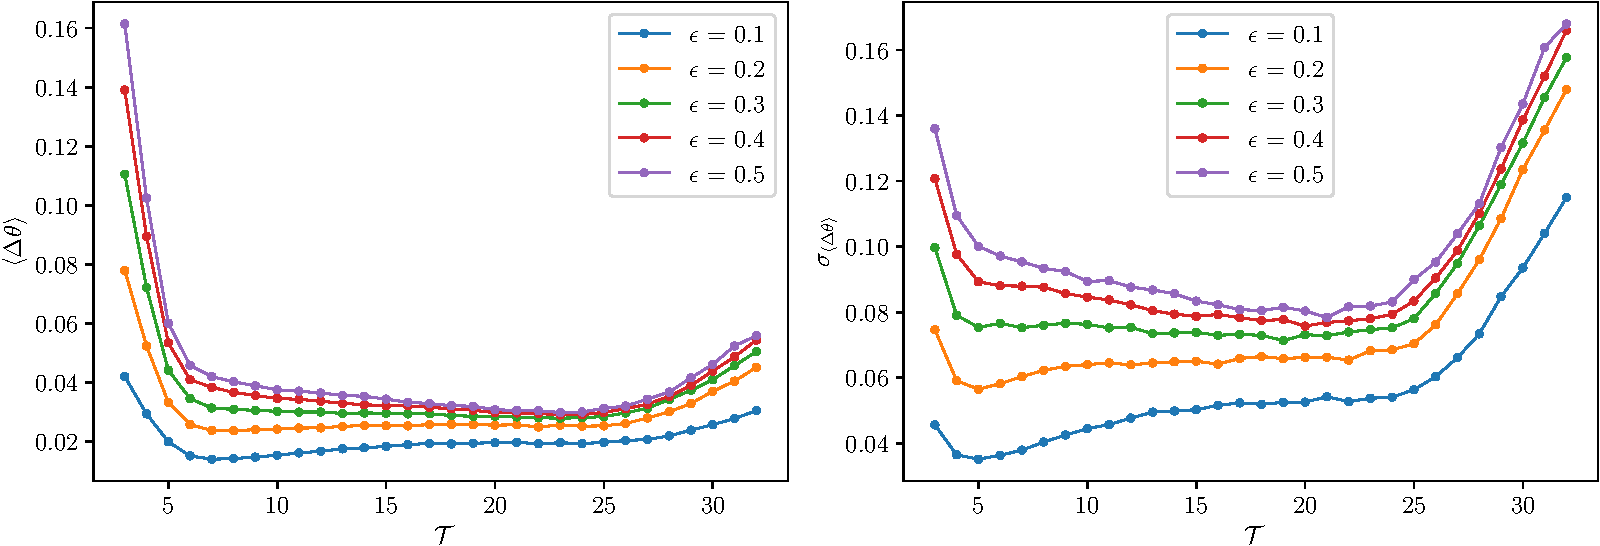
\includegraphics[width=0.9\textwidth]{figures/error_excitable}
    \caption{رفتار خطای نسبی پارامترها در مرز ناحیه غیربرانگیخته و برانگیخته}
    \label{fig:error_excitable}
\end{figure}

همان‌طور که در
\autoref{fig:error_excitable}
مشاهده می‌کنید، با افزایش طول دنباله‌ی مشاهده شده از یک نورون بیمار، مقدار کمینه خطای پارامترها ابتدا به سرعت کاهش یافته و سپس
برای دنباله‌های با طول بیشتر از ۶، در یک بازه نسبتاً طولانی تقریباً ثابت باقی می‌ماند.
این به این معنی است که دنباله‌های با طول بیشتر از ۶ اطلاعات بیشتری از رفتار نورون فراهم نمی‌کنند.
در نتیجه، برای کمینه کردن و تصحیح خطای پارامترها، مشاهده دنباله‌هایی به طول ۶ از دینامیک نورون کافی است.

این طول مشخصه، ممکن است به دو عامل وابسته باشد.
اولین عامل می‌تواند مدت زمان لازم برای گذار نورون به حالت پایدار خود پس از ایجاد خطا در پارامتر‌های مدل باشد.
دومین عامل نیز می‌تواند به مدت زمان یک اسپایک بستگی داشته باشد، زیرا عمده اطلاعات مربوط به دینامیک یک سیستم نورونی در رفتار پتانسیل عمل آن نورون نهفته است.

\subsubsection{مرز بین ناحیه غیربرانگیخته و آشوبناک}

\begin{figure}[!ht]
    \centering
    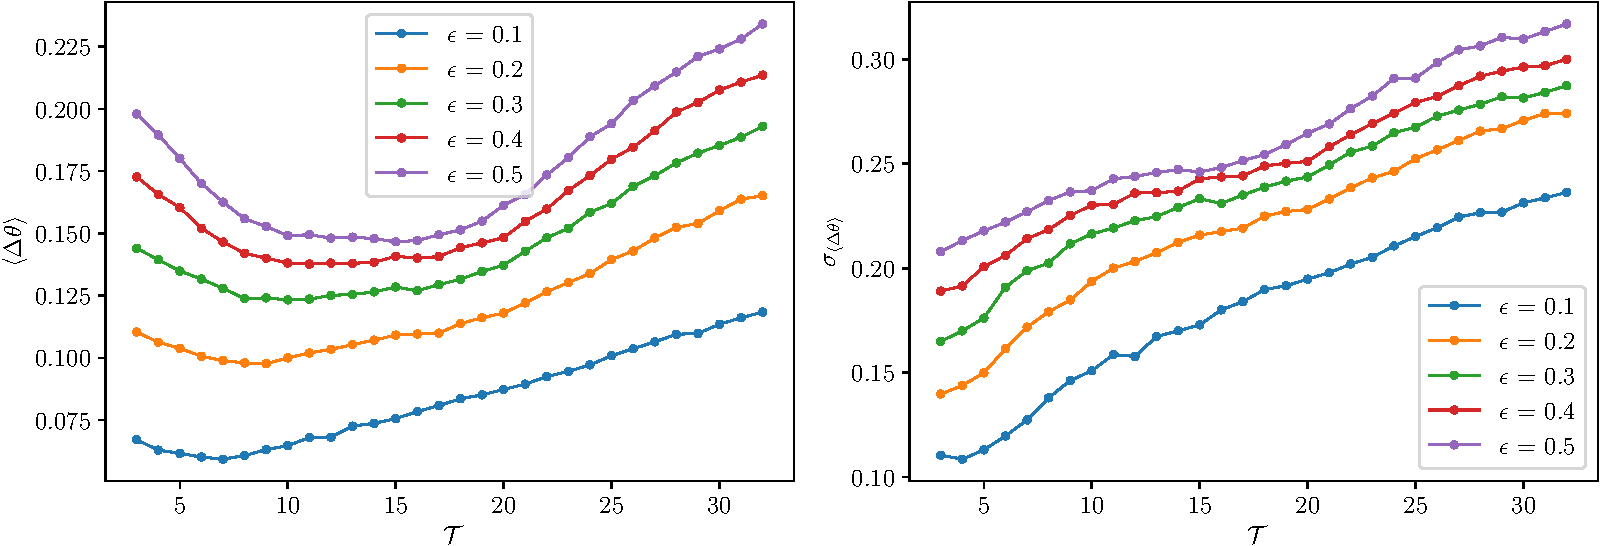
\includegraphics[width=0.9\textwidth]{figures/error_chaotic}
    \caption{رفتار خطای نسبی پارامترها در مرز ناحیه غیربرانگیخته و آشوبناک}
    \label{fig:error_chaotic}
\end{figure}

همان‌طور که در
\autoref{fig:error_chaotic}
مشاهده می‌کنید،
رفتار کمینه خطای پارامترها در این ناحیه با رفتار کمینه خطا در مرز ناحیه برانگیخته متفاوت است.
در اینجا، کمینه خطای پارامترها در ابتدا با افزایش طول دنباله مشاهده شده با شیب بسیار کمتری نسبت به مرز ناحیه برانگیخته کاهش می‌یابد، اما پس از آن و با افزایش بیشتر طول دنباله، خطا افزایش می‌یابد.
این رفتار را می‌توان این چنین توضیح داد که در دنباله‌های کوتاه‌تر، افزایش طول دنباله مشاهده شده اطلاعات بیشتری از رفتار سیستم فراهم می‌کند.
در نتیجه، در ابتدا کاهش خطای پارامترها با افزایش طول دنباله مشاهده شده آسان‌تر است.
اما با افزایش بیشتر طول دنباله مشاهده شده، به دلیل ماهیت آشوبناک سیستم و دور شدن دنباله‌ها به صورت نمایی از یکدیگر، یافتن پارامترهای مناسب دشوارتر شده و مقدار کمینه خطا افزایش می‌یابد.

در این ناحیه، مشاهده دیگری که قابل توجه است، وابستگی طول دنباله‌ی لازم برای رسیدن به کمینه خطا به مقدار اولیه خطای پارامترها است.
به طوری که هر چه خطای اولیه بیشتر باشد، دنباله‌هایی با طول بلندتر برای رسیدن به کمینه خطا نیاز است.
همچنین، مقدار کمینه خطا نیز به خطای اولیه بستگی دارد و هر چه خطای اولیه بزرگتر باشد، مقدار کمینه خطا نیز بزرگتر خواهد بود.
